\documentclass[a4paper,parskip,headheight=38pt]{scrartcl} % article or scrartcl
\usepackage[utf8]{inputenc}
\usepackage[T1]{fontenc}
\usepackage{amsmath,amssymb,amsfonts}
\usepackage[%
  automark,
  headsepline                %% Separation line below the header
]{scrlayer-scrpage}
\usepackage[english]{babel}
\usepackage{hyphenat}
\usepackage[hidelinks]{hyperref}
\usepackage[top=1.4in, bottom=1.5in, left=1in, right=1in]{geometry}
\usepackage{lastpage}
\usepackage{csquotes}
\usepackage{microtype}
\usepackage{datetime}

\usepackage[normalem]{ulem}
\usepackage{enumerate}
\usepackage{hyperref}

\usepackage{microtype}

\usepackage[hang]{footmisc}
\setlength{\footnotemargin}{3mm}

\usepackage{enumitem}

\usepackage[export]{adjustbox}

% \usepackage{multicol}
\usepackage{graphicx}
\usepackage{graphics}
% \usepackage{float}
% \usepackage{caption}

\usepackage{pdflscape}

\parindent 0pt
\parskip 6pt

\clubpenalty = 10000
\widowpenalty = 10000
\displaywidowpenalty = 10000

\renewcommand\thesubsection{\Alph{subsection}}

\setkomafont{pagehead}{\normalfont\sffamily\footnotesize}
\addtolength{\headheight}{+13pt}
\lohead{Marlene Böhmer, s9meboeh@stud.uni-saarland.de, 2547718 \\
	Maximilian Köhl, s8makoeh@stud.uni-saarland.de, 2553525 \\
	Maximilian Schwenger, schwenger@stud.uni-saarland.de, 2542438\\
	Ben Wiederhake, s9bewied@stud.uni-saarland.de, 2541266}
\rohead{
\includegraphics[height=36pt, right]{../logo/logo.png} \newline ES16, Specification, Group 6, Page {\thepage}/{\pageref*{LastPage}}}

\newtimeformat{mytime}{\twodigit{\THEHOUR}\twodigit{\THEMINUTE}\twodigit{\THESECOND}}
\settimeformat{mytime}
\newdateformat{mydate}{\twodigit{\THEYEAR}\twodigit{\THEMONTH}\twodigit{\THEDAY}}
\cfoot{\tiny\texttt{ID \mydate\today\currenttime}}
\chead{} % Needed because now the \subsections get displayed
\pagestyle{scrheadings}

% \renewcommand{\headrulewidth}{0pt}
% \addtolength{\textheight}{+30mm}
% \addtolength{\textwidth}{+50mm}
% \addtolength{\hoffset}{-7mm}

% \newcommand{\Omicron}{\ensuremath{\mathcal{O}}}
% \newcommand{\omicron}{\ensuremath{o}}
% \newcommand{\set}[1]{\{#1\}}
% \newcommand{\abs}[1]{\lvert #1 \rvert}

\DeclareMathOperator{\sinc}{sinc}

\begin{document}
We wrote our own library which contains custom blocks that allow us to build simulations. Because of the complexity of the whole system we decided to use a unit-test-like approach to test specific components.

You will find an overview over all customs blocks in the library file itself which is also attached at the end of this document for convenience.

\section{Environment}
Because there is no pre-built block in Simulink which would suffice for the environment, we needed to come up with our own approach. The maze and all entities in it are described in a text file which is loaded into Matlab and transformed into a matrix. This matrix represents the entire environment and is used in raycast computations to determine sensor readings of the proximity sensors and IR sensors at a given point in time and space. This happens within our custom sensor blocks.

E-Puck's motor is realized by a custom \emph{Differential Drive} Block implementing the real world physics by using adequate differential equations. The block assures that the Tin Bot cannot drive through other objects by looking up the occupation status in the matrix and restricting the motion appropriately.

The complete physical Tin Bot is represented by the block \emph{Tin Bot Physical}. This block feeds the differential drive's data (position and orientation) in the appropriate sensor blocks — taking the orientation offset of the sensors into account — such that their values can be computed appropriately using raycasting.

According to the Tin Bot's current position given by the differential drive, the matrix is updated such that Tin Bots cannot drive through each other. Therefore, a \emph{Tin Bot Introducer} block has to be connected to the block representing the physical Tin Bot. This block writes an appropriate value in the matrix at the Tin Bot's current position. To use multiple Tin Bots within the simulation, the Introducer blocks are chained such that at the end there is a matrix containing all the Tin Bots.

The map used by the Tin Bot's sensors, however, must not contain its own Tin Bot. Therefore, the \emph{Tin Bot Eliminator} block deletes the respective entry from the environment. This prevents the sensors from detecting themselves.

The \emph{LPS} block takes the environment's data and feeds it into the Tin Bots every two seconds. This data is then used within the software blocks. The LPS block allows for two states, enabled and disabled, as described in our specification document.

The \emph{Victim Introducer} block uses a similar mechanism as the Tin Bot Introducer, to place the victim inside the matrix representing the map. The \emph{Victim} block participates in a loop which models the picking up process by a Tin Bot.

The output of the control software is fed back to the environment, which allows us to model real world physics.

\section{Components}
In the following description of our components we define the term \enquote{\emph{introduce}} as recording the position of an object in the matrix representing the environment by setting a certain value in the particular cell(s) the object is located in.

\subsection{Physical Environment}
\subsubsection{Tin Bot Introducer}
Records the position of the Tin Bot inside the matrix representing the environment. Because the matrix is used as input for the drives again the Block delays the position by one sample to prevent algebraic loops using \emph{x0} respectively \emph{y0} as starting position.
\begin{description}
\item[Inputs:] \hfill
	\begin{description}
	\item[row\_in] Current row the Tin Bot should be placed in.
	\item[col\_in] Current column the Tin Bot should be placed in.
	\item[reset] (Not used in our simulation, resets the internal state.)
	\item[x0] Starting position of the Tin Bot.
	\item[y0] Starting position of the Tin Bot.
	\item[map\_in] Matrix representing the environment without the corresponding Tin Bot.
	\end{description}
\item[Outputs:] \hfill
	\begin{description}
	\item[map\_out] Matrix representing the environment with the corresponding Tin Bot.
	\item[row\_out] Row where the Tin Bot has been introduced (delayed).
	\item[col\_out] Column where the Tin Bot has been introduced (delayed).
	\end{description}
\end{description}

\subsubsection{Tin Bot Eliminator}
\begin{description}
\item[Inputs:] \hfill
	\begin{description}
	\item[map\_in] Matrix representing the environment (all objects have to be introduced).
	\item[row] Row where the corresponding Tin Bot has been introduced.
	\item[col] Column where the corresponding Tin Bot has been introduced.
	\end{description}
\item[Outputs:] \hfill
	\begin{description}
	\item[map\_out] Matrix representing the environment without the corresponding Tin Bot.
	\end{description}
\end{description}

\subsubsection{Victim Introducer}
\begin{description}
\item[Inputs:] \hfill
	\begin{description}
	\item[map\_in] Matrix representing the environment without the victim.
	\item[victim] Current position of the Victim as 2 dimensional vector ($[x\,\, y]$). 
	\end{description}
\item[Outputs:] \hfill
	\begin{description}
	\item[map\_out] Matrix representing the environment with the victim.
	\end{description}
\end{description}

\subsubsection{IR Sensor}
Implementing an IR sensor using raycasting.


\subsubsection{Proximity Sensor}
\subsubsection{Differential Drive}
\subsubsection{Differential Drive Restricted}

\subsection{Software}
Besides the model of the environment, there are various other components mainly modeling the software running on the Tin Bot as Stateflow charts.

\subsubsection{Tin Bot Approximator}

This component takes the driving information (which wheels turn how
quickly), and the occasional update via LPS, and approximates the
current position and orientation from it.

FIXME

\subsubsection{Traffic Cop Eyes}

Detects good points in time to measure the exact angle to the victim,
and interrupts \enquote{Traffic Cop} (see below) to start the
measurement.

\begin{description}
\item[Inputs:] \hfill
	\begin{description}
	\item[current\_x\_y\_phi] Approximate position and orientation of the Tin Bot. 
	\item[ir\_raw] Current IR sensor readings.
	\item[found\_victim\_phi] Flag to indicate that new angular information is available.
	\item[found\_victim\_xy] Flag to indicate that new cartesian information is available.
	\end{description}
\item[Outputs:] \hfill
	\begin{description}
	\item[need\_angle] Whether a new angular measurement should be taken.
	\end{description}
\end{description}

\subsubsection{Victim Direction}

This component is responsible for measuring and computing the precise angle to the victim.

\begin{description}
\item[Inputs:] \hfill
	\begin{description}
	\item[ir] Current IR sensor readings.
	\item[current\_x\_y\_phi] Approximate position and orientation of the Tin Bot. 
	\item[run\_finder] Flag whether this subsystem shall be active.
	\end{description}
\item[Outputs:] \hfill
	\begin{description}
	\item[mot\_l, mot\_r] Motor instructions.
	\item[found\_victim] Flag to indicate that \emph{v\_phi} can be read.
	\item[v\_phi] If flag is set, this is the absolute angle to the victim, as per the most recent measurement.  Otherwise, garbage.
	\end{description}
\end{description}

\subsubsection{Victim Detector}

This component is responsible for taking angular measurements, and
triangulating them to a concrete coordinates of the victim.

\begin{description}
\item[Inputs:] \hfill
	\begin{description}
	\item[found\_victim\_phi] Flag to indicate that \emph{victim\_angle} can be read.
	\item[victim\_angle] If flag is set, this is the absolute angle to the victim, as per the most recent measurement.  Otherwise, garbage.
	\item[current\_x\_y\_phi] Approximate position and orientation of the Tin Bot. 
	\end{description}
\item[Outputs:] \hfill
	\begin{description}
	\item[found\_victim\_xy] Flag to indicate that \emph{victim\_x, victim\_y} can be read.
	\item[victim\_x, victim\_y] If flag is set, this are the coordinates of the victim.  Otherwise, garbage.
	\end{description}
\end{description}

\subsubsection{Right Hand Follower}

This is the default model of operation,  which does not keep track of
previous locations, but just applies the right hand rule until another
component has a better idea what to do.

\begin{description}
\item[Inputs:] \hfill
	\begin{description}
	\item[run\_rhr] Flag whether this subsystem shall be active.
	\item[proximity] Current proximity sensor readings (8-dimensional vector).
	\end{description}
\item[Outputs:] \hfill
	\begin{description}
	\item[motor\_left, motor\_right] Motor instructions.
	\end{description}
\end{description}

\subsubsection{Sensor Filter}

This component \enquote{filters} the sensor inputs for Path Finder (see
below), so that the victim is not recognized as an obstacle.  (Since it
is \enquote{docked} to the back of the Tin Bot, this can't cause the
Tin Bot to drive into a wall.)

\begin{description}
\item[Inputs:] \hfill
	\begin{description}
	\item[ir] Current IR sensor readings (6-dimensional vector).
	\item[proximity\_in] Current proximity sensor readings (8-dimensional vector).
	\end{description}
\item[Outputs:] \hfill
	\begin{description}
	\item[proximity\_out] Filtered proximity sensor readings (8-dimensional vector).
	\end{description}
\end{description}

\subsubsection{Path Finder}
As soon as the Tin Bot knows the location of the victim, the reminder of the problem is basically a maze solving task under a partially known maze. 
Path Finder takes care of computing the waypoints leading to the victim at first, and out of the maze when the victim has been picked up. 

Note that Path Finder constantly collects information about the environment, even if $compute$ is cleared.

\begin{description}
\item[Inputs:] \hfill
    \begin{description}
    \item[proximity] Filtered proximity sensor readings (8-dimensional vector).
    \item[current\_x\_y\_phi] Approximate position and orientation of the Tin Bot.
  	\item[dst\_x, dst\_y] Destination location (either victim or nearest exit).
    \item[compute] Flag whether this subsystem shall be active.
	\end{description}
\item[Outputs:] \hfill
	\begin{description}
    \item[drive] Flag whether the Path Executor subsystem shall be active.
    \item[next\_x, next\_y] Next waypoint.
    \item[no\_path] Flag whether $A^\ast$ search has failed, and some fallback system needs to run.
    \item[path\_completed] Flag whether the Path Finder and Path Executor subsystems is done.
	\end{description}
\end{description}

\subsubsection{Path Executor}

The Path Executor tries to reach each waypoint directly, i.e.\ drives straight to the given point. 

\begin{description}
\item[Inputs:] \hfill
    \begin{description}
    \item[drive] Flag whether this subsystem shall be active.
    \item[current\_x\_y\_phi] Approximate position and orientation of the Tin Bot.
  	\item[dest\_x, dest\_y] Destination location (next waypoint).
	\end{description}
\item[Outputs:] \hfill
	\begin{description}
	\item[wheel\_left, wheel\_right] Motor instructions.
	\end{description}
\end{description}

\subsubsection{Blind Traffic Cop}

Decide \enquote{who is allowed to drive}, and keep track of overall Tin Bot state.

\begin{description}
\item[Inputs:] \hfill
    \begin{description}
    \item[need\_angle] Flag whether this subsystem shall be active.
	\item[found\_victim\_phi] Flag to indicate that new angular information is available.
    \item[found\_victim\_xy] Flag to indicate that new cartesian information is available.
    \item[no\_path] Flag whether $A^\ast$ search has failed, and some fallback system needs to run.
    \item[path\_completed] Flag whether the Path Finder and Path Executor subsystems is done.
	\item[victim\_x, victim\_y] If corresponding flag is set, this are the coordinates of the victim.  Otherwise, garbage.
	\item[initial\_x, initial\_y] Start coordinates (needed as exit).
	\end{description}
\item[Outputs:] \hfill
	\begin{description}
  	\item[dst\_x, dst\_y] Destination location (either victim or nearest exit).
    \item[run\_path\_finder] Flag whether the Path Finder/Executor subsystems shall be active.
	\item[run\_rhr] Flag whether the right-hand rule subsystem (Right Hand Follower) shall be active.
	\item[run\_victim\_finder] Flag whether the Victim Direction subsystem shall be active.
	\end{description}
\end{description}

\subsubsection{Traffic Cop}

Wrapper for Blind Traffic Cop and Traffic Cop Eyes.

\subsection{Communications}

\subsubsection{LPS}

FIXME

FIXME

\subsection{Abstractions and Compositions}
\subsubsection{Tin Bot Controller}

Wrapper for the following components: \\
Victim Direction, Victim Detector, Follow Right Hand, Sensor Filter, Path Finder, Path Executor, Traffic Cop

\subsubsection{Tin Bot Software}

Wrapper for the following components: \\
Tin Bot Controller, Tin Bot Approximator

\subsubsection{Tin Bot Abstraction}
\subsubsection{Tin Bot}
\subsubsection{Victim}

% ------


Next, there is the detection of good points in time to measure the exact angle to the victim.  We assume that the intersection of all measurements provides a reasonably good result.  This functionality is spread across \emph{Traffic Cop Eyes, Victim Finder, Victim Detector}; each of which are state machines.


All these modules, who in composition are called \emph{Controller}, need the concept of \enquote{current location and direction}, which is given by the \emph{Approximator}. This module takes the LPS data (if available) and motor output, and tries to interpolate the current position and direction from it. This module applies the same differential equations as the Differential Drive.

\section{Test Cases}
As already mentioned we mostly used a unit-test-like approach to test all aspects of the system, only the last two tests cover the combination of the system components.

\subsection{Unit-Tests}
\begin{description}
\item[drive\_test] Tests the physical model of differential drive isolated from any logic.
\item[proximity\_test] Tests the physical model of the proximity sensors separately. % note that there is no adverb for isolated, thus separately
\item[ir\_test] Tests the physical model of the IR sensors of the Tin Bot.
\item[traffic\_blind\_test] Tests the \enquote{blind} part of the traffic cop, i.e.\ without any IR-sensor input.
\item[victim\_direction\_test] Tests victim direction calculation, i.e.\ the logic used to approximate the angle from the Tin Bot to the victim based on IR-sensor input.
\item[path\_finder\_test] Tests internal map generation and escape path calculation, i.e.\ in essence also a test for \textbf{UC-D}, since one can see that the logic is able to deal with formerly unknown obstacles and behave reasonably.
\item[approximator\_test] Tests approximation of current position and orientation based on the motors data as opposed to real data provided by the LPS. Also checks update mechanism in case the LPS is turned on.
\item[follow\_right\_hand\_test] Tests the correct application of the right hand rule taking proximity sensor data into account. Covers large parts of the project since most components are involved.
\end{description}

\subsection{System-Test}
The test \textbf{controller\_test} implements the concrete virtual prototype. It tests the complete control software within the simulated environment and use cases \textbf{UC-D}, \textbf{UC-E} and \textbf{UC-F} as well as requirements \textbf{MR2}, \textbf{MR4}, \textbf{MR5}, \textbf{MR6}, \textbf{MR8}, \textbf{MR10}, \textbf{NR1}, \textbf{NR4}, \textbf{MR14}, \textbf{MR15}, \textbf{MR16}, \textbf{MR17}, \textbf{NR7}. 

% <TODO: implement use case C by bypassing the map chain> -> nice to have, not necessary

Use cases \textbf{UC-A} and \textbf{UC-B} are modeled implicitly, because startup corresponds to starting the simulation, and shutdown corresponds to stopping the simulation.
Use case \textbf{UC-C} corresponds to a nice-to-have feature and is not modeled. We did, however, not yet model tests with more than one Tin Bot at a time, so the failure of one has no impact anyways.

\newgeometry{top=2cm,bottom=2cm,right=2cm,left=2cm}
\pagestyle{empty}

\begin{landscape}
\begin{figure}[h]
\centering
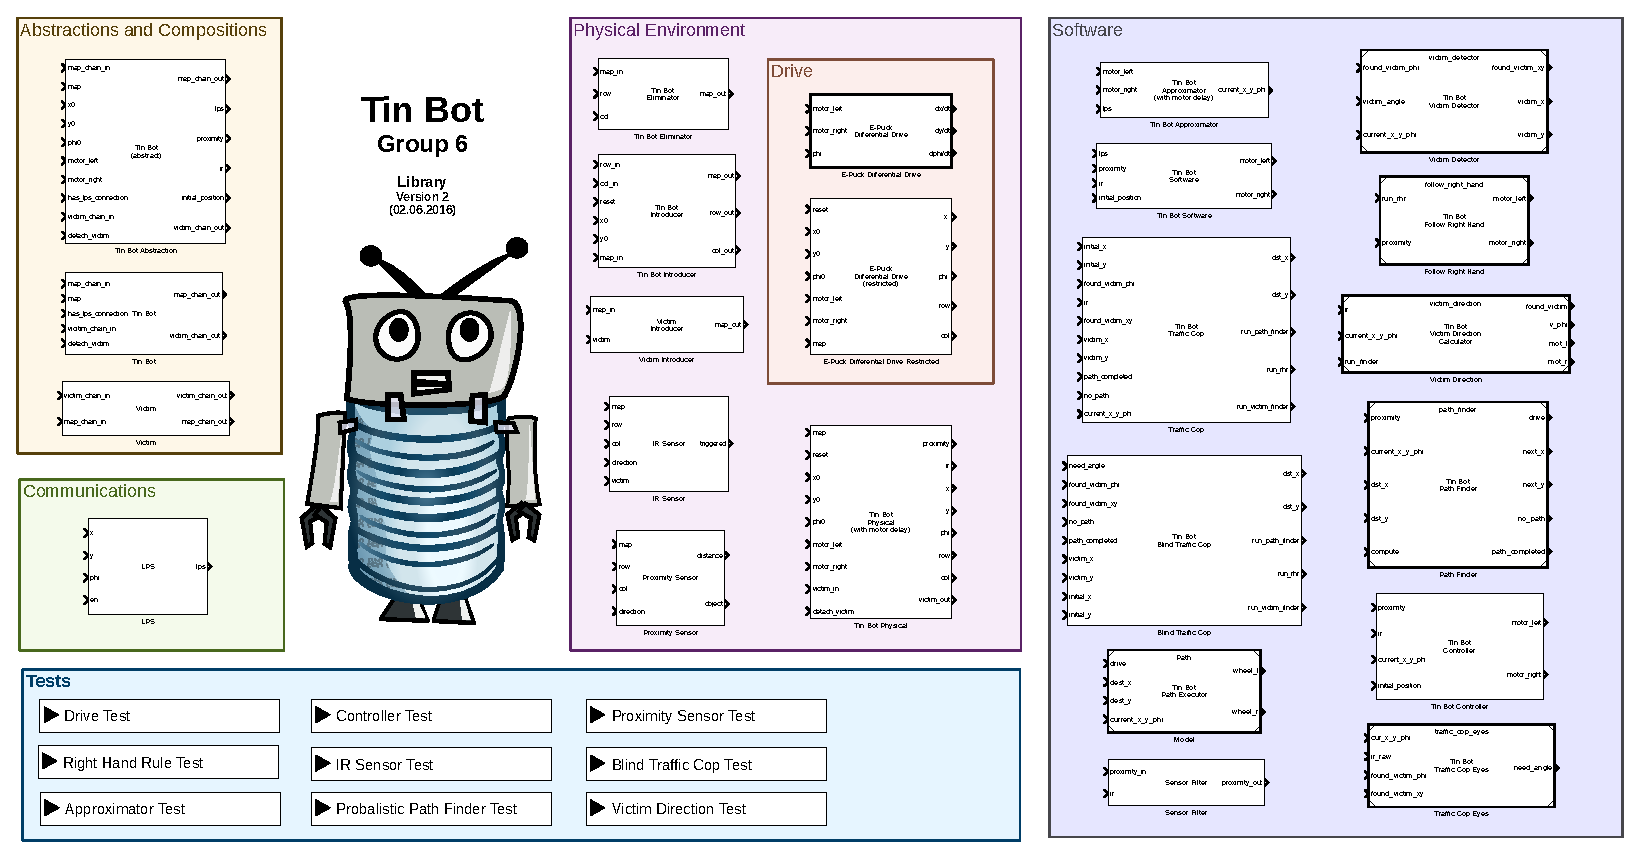
\includegraphics[width=26cm]{library.pdf}
\label{}
\end{figure}
\end{landscape}

\end{document}
